\documentclass{article}
\usepackage{listings}
\usepackage{amsmath}
\usepackage{fullpage}
\usepackage{graphicx}
\usepackage{wrapfig}
\usepackage[
	colorlinks=true,
	urlcolor=black,
	linkcolor=blue,
	citecolor = black,
	naturalnames=true,
	pdftitle={LIMES Webservice},
	pdfsubject={Manual},
	pdfauthor={Klaus Lyko},
	pdfkeywords={LIMES, Link Discovery, Linked Data, Webservice}
]{hyperref}
%%%%%%%%%%%%%%%%%%%%%%%%%%%%%%%%%%%%%%%%%%%%%%%%%%%%
\begin{document}

%\thispagestyle{empty}
% titlepage
\begin{titlepage}
	\begin{center}
		% Upper part of the page
		
\includegraphics[width=\textwidth]{images/limes_logo.pdf}
		\centering
		\huge Limes Webservice User Manual
		\huge Version 0.1	
		\vfill
		% Bottom of the page
	%	\large \today
	\end{center}
\end{titlepage}
\tableofcontents
%%%%%%%%%%%%%%%%%%%%%%%%%%%%%%%%%%%%%%%%%%%%%%%
\newpage
\section{Introduction}
This document describes the LIMES Webservice (LWS).\\
LWS was developed as a student project at the University of Leipzig in 2012 and is currently maintained by Klaus Lyko at the 
Note that LWS is still under development. Hence, all describes features are in a beta status.

\subsection{Deployed version}
We deployed the current stable LWS version at: \url{http://139.18.2.164:8080/axis2/services/LimesServiceImpl} \\
The prebuild sample client could be downloaded at \url{139.18.2.164:8080/LimesWebService_Client.jar}.\\
If you notice some bugs feel free to post them at our GitHub reporsitory: \url{https://github.com/KLyko/LimesWebService/}

\section{The Webservice}
This section describes the features and basic architecture of the LWS.
\subsection{Features}
\begin{figure}[htbp]
	\centering
		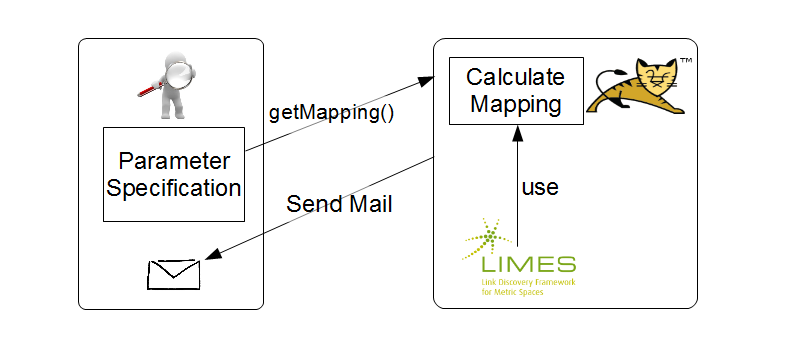
\includegraphics[width=7in]{images/limes_webservice_workflow_skizze_for_dummies.png}
	\caption{Basic workflow}
	\label{fig:limes_webservice_workflow_skizze_for_dummies}
\end{figure}
The main purpose of LWS is to profide a Webservice to use the LIMES mapping mechanisms. Given a so-called Link Specification LWS profides the getMapping() method, which basically runs the LIMES framework with the given specifications. As the mapping process can last some time (above all querying large and/or slow endpoints) the method is designed asnychronous: Once, LIMES has finished calculation the Webservice  will send an email with the results as attachement. Therefore, above all LWS expects that the user submitted ancemail address results will be send to.
Figure~\ref{fig:limes_webservice_workflow_skizze_for_dummies} depicts the basic workflow of LWS. First a client has to start a session, submitting parameters such as an email address and the neccessary LIMES Link Specification parameters. Finally, the client calls the getMapping() method to start the linking process. Once the server finishes calculation it sends the results as an email attachement. Figure~\ref{fig:workflow2} illustrates all these major methods and usecases of LWS.
\begin{figure}[h]
	\centering
		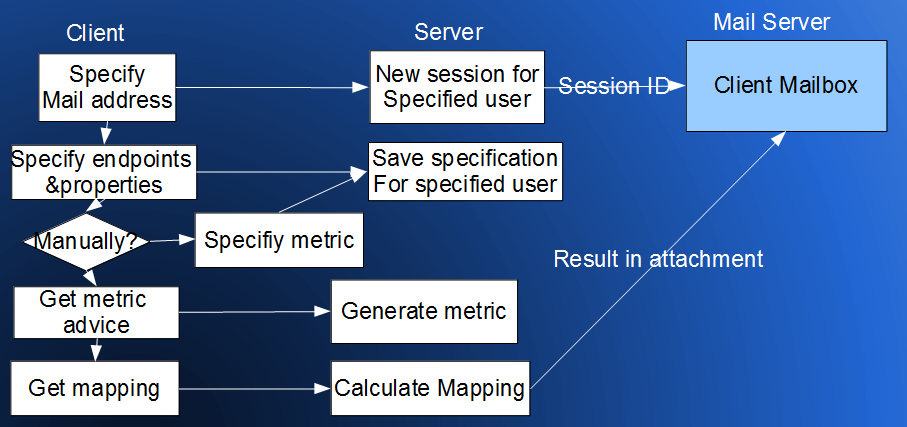
\includegraphics[width=7in]{images/workflow2.png}
	\caption{Workflow of LWS}
	\label{fig:workflow2}
\end{figure}

\subsection{Architecture}
We developed a basic Webservice using the Apache Axis2\footnote{\url{http://axis.apache.org/axis2/java/core/}} framework. 

%%%%%%%%%%%%%%%%%%%%%
\section{The Client}
A client working for LWS was build with JAVA and can be downloaded as a pre-buildt jar at \url{https://github.com/KLyko/LimesWebService/}.

\end{document}